%% Praktikos veiklos aprašymas (vienas arba keli skyriai). Aprašomas praktikos užduoties įgyvendinimas (pvz., atlikti projektavimo ir/ar programavimo darbai, sukurtas modelis, priimti sprendimai ir pan.).

\section{PROFESINĖS PRAKTIKOS VEIKLA}
\label{praktikos_veiklos_aprasymas}

Profesinę praktiką sudarė trys užduotys:
\begin{enumerate}
 \item Susipažinti su matų atrinkimo daugiamačiuose duomenyse problematika bei moksline literatūra;
 \item Suprogramuoti matų atrinkimo metodus;
 \item Ištirti matų atrinkimo metodų savybes.
\end{enumerate}
Toliau aprašau kiekvieną užduotį atskirai.

\subsection{Matų atrinkimas daugiamačių duomenų klasifikavimui}

Savo bakalauriniame darbe yra nagrinėju biomedicinoje kaupiamų genetinių daugiamačių duomenų analizės specifiką. Šie duomenys yra specifiški tuo, kad jie turi šimtus kartų daugiau matų nei mėginių. Kadangi mėginio gavimo kaina yra aukšta, turimas mažas mėginių skaičius turimas. Biomedicininių duomenų analizę apsunkina ir tai, kad matavimai, kuriais tie duomenys gaunami, yra triukšmingi. Triukšmas matavimo metu atsiranda dėl cheminių reakcijų netikslumo, tiriamo organizmo sudėtingumo. Kai duomenys yra triukšmingi ir didėja juos apibūdinančių matų skaičius, didėja tikimybė duomenyse rasti atsitiktinių priklausomybių. Tai yra pagrindinė priežastis, kodėl biomedicininių duomenų analizės procesas yra sudėtingas.

Biomedicininių duomenų klasifikavimo užduotis yra atskirti sveikų pacientų mėginius nuo sergančiųjų. Klasifikavimu siekiama nustatyti, kurie matai, veikdami drauge, geriausiai paaiškina skirtumą tarp ligos paveiktų ir sveikų mėginių. Labiausiai ligą paaiškinančių matų nustatymas galėtų palengvinti tiriamų ligų diagnozės ir gydymo metodų kūrimą. Klasifikavimu yra vadinamas duomenų analizės procesas, kurio metu yra sukonstruojama funkcija, atskirianti duomenis į grupes pagal jų matus \cite{fisher1936use}. Sukonstruotos funkcijos yra vadinamos klasifikatoriais, o jų konstravimo algoritmai -- klasifikavimo algoritmais. Klasifikatoriai paruošiami naudojant turimus mėginius -- treniravimosi duomenis -- ir informaciją apie jų būklę (sveikas ar sergantis). Klasifikatoriaus ruošimo procesas yra vadinamas apmokymu. Klasifikatoriai paprastai naudojami nustatant naujų, dar nematytų, mėginių būklę. 

Dėl ,,daugiamatiškumo prakeiksmo`` (angl. \textit{the curse of dimentionality}) -- didėjant matų kiekiui mėginiai pasidaro panašūs, todėl bandymas juos klasifikuoti tolygus spėliojimui \cite{bellman1966adaptive}. Biomedicininių duomenų kontekste galima daryti prielaidą, kad ne visi matai yra susiję su tiriama problema, pvz. gaubtinės žarnos vėžiu, dėl to, kad duomenys yra daugiamačiai. Paprastai nagrinėjamai problemai svarbus yra mažas, palyginus su visu, matų kiekis.  Todėl biomedicininių duomenų daugiamatiškumui sumažinti yra naudojami informatyviausių matų atrinkimo metodai \cite{guyon2003introduction} (angl. \textit{feature selection}). Pagal tai, kaip susiję su klasifikatoriumi, matų atrinkimo metodai skirstomi į tris kategorijas \cite{saeys2008robust}: filtruojantys (angl. \textit{filter}), prisitaikantys (angl. \textit{wrapper}) ir įterptiniai (angl. \textit{embedded}) metodai. Filtruojančiais metodais pirmiausia yra atrenkamos informatyviausi matai, o tada apmokomas klasifikatorius. Prisitaikančiųjų metodų atveju, pirma, apmokomas klasifikatorius su visais matais, antra, parenkamas matų poaibis ir apmokomas klasifikatorius, tada po daugkartinio matų aibių įvertinimo pagal klasifikavimo rezultatus yra nusprendžiama, kuris matų poaibis yra labiausiai tinkamas klasifikavimui. Įterptinių metodų atveju matų atrinkimo procesas yra neatsiejamas nuo klasifikavimo proceso -- pats klasifikatorius įvertina matus.

Matų atrinkimas yra svarbi biomedicininių duomenų apdorojimo (angl. \textit{preprocessing}) etapo dalis. Naudojant matų atrinkimo metodus, galima kovoti su daugiamatiškumo prakeiksmu matų skaičių priartinant prie mėginių skaičiaus. Todėl svarbu yra pasirinkti geriausiai tinkančią matų atrinkimo strategiją. Kadangi ir pačių matų atrinkimo metodų veikimas priklauso nuo konkrečių duomenų, tai metodo pasirinkimas yra sudėtinga užduotis.

Naudodami matų atrinkimo metodus, biomedicininius duomenis tiriantys mokslininkai susiduria su atrinktųjų matų aibės stabilumo problema -- atrenkant matus pagal kitą mėginių poaibį, gaunamas kitas matų poaibis. Matų atrinkimo nestabilumas yra sąlygotas šių veiksnių:
\begin{enumerate}
 \item Duomenys yra triukšmingi ir kai kurie matai gali būti palaikyti informatyviais vien dėl atsitiktinių priežasčių;
 \item Daugiamačiuose duomenyse tikėtina, kad dalis matų koreliuoja tarpusavyje, todėl, kuris iš koreliuojančių matų bus pasirinktas, priklauso nuo to, kuriuos mėginius pasirinksime klasifikatoriaus apmokymui;
 \item Kiekvienas matų atrinkimo algoritmas daro skirtingas prielaidas apie tai, kurie matai yra informatyvūs.
\end{enumerate}
Galime daryti išvadas, kad skirtingi metodai tiems patiems duomenims gali atrinkti skirtingus matus. Taip pat, suskaidžius turimus duomenis į atskiras persidengiančias aibes ir atrinkus tą patį kiekį matų tuo pačiu metodu, gaunamos skirtingos matų aibės. Be to, kuo triukšmingesni duomenys, kuo mažiau turima mėginių ir kuo daugiau yra matų, tuo ryškesnė yra ši problema \cite{loscalzo2009consensus}.

Matų atrinkimo stabilumo problemą pirma siūlyta spręsti surandant matų grupių tankio centrus ir naudoti matus, kurie artimiausi tiems centrams \cite{yu2008stable}. Pasiūlytas grupių tankių algoritmas užtrunka $O(\lambda n^2m)$ laiko, kur $n$ yra matų kiekis, o $m$ -- mėginių skaičius. Vėliau Loscalzo ir kt. pasiūlė mokymo duomenis skaidyti poaibiais ir kiekviename poaibyje ieškoti tankių matų grupių, o tada imti sprendimą balsavimo principu \cite{loscalzo2009consensus}. Nors šie metodai siūlo stabilų matų atrinkimą, tačiau jų panaudojamumą daugiamačiuose duomenyse riboja skaičiavimo sudėtingumas.

Yang ir Mao pasiūlė reitinguoti matus remiantis keletos matų atrinkimo metodų rezultatais \cite{yang2011robust}. Galutinis matų reitingų sąrašas gaunamas, kai po kiekvieno matų atrinkimo yra išmetama vienas žemiausią reitingą turintis matas iš matų aibės, ir matų atrinkimas yra kartojamas tol, kol nebelieka matų. Tačiau ši matų atrinkimo strategija yra ribota, nes matų atrinkimo metodų kiekis yra ribotas ir skirtingų metodų dažnai negalima atlikti išskirstytų skaičiavimų aplinkoje. Tai riboja šio metodo pritaikomumą daugiamačių duomenų analizėje.

Praktikos metų išstudijavau esamus stabilių matų atrinkimo metodus nustačiau, kad jie tik šiek tiek padidina matų atrinkimo stabilumą, bet problemos iš esmės neišsprendžia.

\subsection{Suprogramuoti matų atrinkimo algoritmai}

Profesinės praktikos metu suprogramavau populiariausius matų atrinkimo metodus. Taip pat programavau ir matų atrinkimo stabilumą didinančius metodus. Toliau šiame poskyryje aprašau šiuos metodus.

\subsubsection{\textit{Fisher} įvertis}

\textit{Fisher} įvertis vertina individualius matus pagal matų klasių atskiriamąją galią. Mato įvertis yra sudarytas iš tarpklasinio skirtumo santykio su vidiniu klasės pasiskirstymu:
\begin{equation}
 FR(j) = \frac{(\mu_{j1} - \mu_{j2})^2}{\sigma_{j1}^2 + \sigma_{j2}^2},
\end{equation}
kur, 
$j$ -- yra mato indeksas, 
$\mu_{jc}$ -- mato $j$ reikšmių vidurkis klasėje $c$, 
$\sigma_{jc}^2$ -- mato $j$ reikšmių standartinis nuokrypis klasėje $c$, kur $c={1,2}$. Kuo didesnis yra \textit{Fisher} įvertis, tuo geriau ts matas atskiria klases. Nors ir paprastas, šis metodas neįvertina matų tarpusavio sąveikų.

\subsubsection{\textit{Relief} metodas}

\textit{Relief} metodas iteratyviai skaičiuoja matų ,,susietumą``. Pradžioje ,,susietumas`` visiems matams yra lygus nuliui. Kiekvienoje
iteracijoje atsitiktinai pasirenkamas mėginys iš mėginių aibės, surandami artimiausi kaimynai iš tos pačios ir kitos klasės, ir atnaujinamos visų 
matų ,,susietumo`` reikšmės. Dėl atsitiktinumo faktoriaus klasifikavimo ir  matų atrinkimo stabilumo rezultatai naudojant šį metodą varijuoja. Mato įvertis yra vidurkis visų objektų atstumų skirtumų iki artimiausių kaimynų iš kitos ir tos pačios klasių:
\begin{equation}
 W(j)=W(j) - \frac{diff(j, x, x_H)}{n} + \frac{diff(i, x, x_M)}{n},
\end{equation}
kur 
$W(j)$ -- $j$-ojo mato ,,susietumo`` įvertis, 
$n$ -- mėginių aibės dydis, 
$x$ -- atsitiktinai pasirinktas mėginys, 
$x_H$ - artimiausias $x$ kaimynas iš tos pačios klasės (angl. \textit{nearest-Hit}), 
$x_M$ -- artimiausias $x$ kaimynas iš kitos klasės(angl. \textit{nearest-Miss}),
$diff(j, x, x')$ -- $j$-ojo mato reikšmių skirtumas tarp laisvai pasirinkto objekto $x$ ir atitinkamo kaimyno, kur skirtumą į intervalą $[0, 1]$ normalizuojanti funkcija yra:
\begin{equation}
 diff(j, x, x')=\frac{|x_j- x_j'|}{x_{j_{max}} - x_{i_{min}}},
\end{equation}
kur $x_{j_{max}}$ ir $x_{j_{min}}$ yra maximali ir minimali $j$-ojo matų reikšmės. ,,Susietumo`` reikšmių atnaujinimas yra vykdomas $n$ kartų ir kuo didesnė galutinė reikšmė, tuo svarbesnis matas. Aprašyta algoritmo versija yra skirta dviejų klasių atvejui, tačiau yra ir multiklasinis algoritmo variantas.

\subsubsection{Asimetrinis priklausomybės koeficientas}

Asimetrinis priklausomybės koeficientas (angl. \textit{asymetric dependency coefficient}, ADC) yra matų reitingavimo motodas, kuris matuoja mėginio grupės tikimybinę priklausomybę $j$-ajam matui, naudodamas informacijos prieaugį (angl. \textit{information gain}) \cite{kent1983information}:
\begin{equation}
 ADC(Y, j) = \frac{MI(Y, X_j)}{H(Y)},
\end{equation}
kur $H(Y)$ -- klasės $Y$ entropija (angl. \textit{entropy}), o $MI(Y, X_j)$ -- yra tarpusavio informacija \cite{Shannon:2001:MTC:584091.584093} (angl. \textit{mutual information}) tarp mėginio grupės $Y$ ir $j$-ojo mato.
\begin{equation}
 H(Y)=-\sum_y{p(Y=y)log{p(Y=y)}}, 
\end{equation}
\begin{equation}
 H(X_j)=-\sum_x{p(X_j=x) log{p(X_j=x)}},
\end{equation}
\begin{equation}
 MI(Y, X_j) = H(Y) + H(X_j) - H(Y, X_j),
\end{equation}
\begin{equation}
 H(Y, X_j) = -\sum_{y,x_j}{p(y, x_j)log{p(y, x_j)}},
\end{equation}
Kuo didesni ADC įverčiai, tuo matas yra svarbesnis, nes turi daugiau informacijos apie mėginio priklausomybę grupei.

\subsubsection{Absoliučių svorių SVM}

Atraminių vektorių metodas (SVM) yra vienas populiariausių klasifikavimo algortimų, nes jis gerai susidoroja su daugiamačiais duomenimis \cite{guyon2002gene}. Yra keletas bazinių SVM variantų \cite{vapnik2000nature}, bet šiame darbe naudosime tiesinį SVM, nes jis demonstruoja gerus rezultatus analizuojant genų ekspresijos duomenimis. Tiesinis SVM yra hiperplokštuma apibrėžta kaip:
\begin{equation}
 \sum_{j=1}^{p}{w_jx_j + b_0 = 0},
\end{equation}
kur $p$ -- dimensijų kiekis, $w_j$ -- j-osios dimensijos svoris, $x_j$ -- j-osios
dimensijos kintamasis, $b_0$ -- konstanta. Dimensijos absoliutus\footnote{Svorį
reikia imti absoliutaus dydžio, nes neigiamas svoris implikuoja priklausomybę 
vienai klasei, o teigiamas kitai klasei.} svoris $w_j$ gali būti panaudotas
dimensijų reitingavimui. Pastebėtina, kad svorių nustatymas yra atliekamas tik 
vieną kartą\footnote{SVM-RFE dimensijų atrinkimo metodas svorius nustato daug kartų.}.


\subsection{Suprogramuotų dimensijų atrinkimo algoritmų palyginimas}

\subsubsection{Dimensijų atrinkimo algoritmų skaičiavimo laikas}

Eksperimentai buvo atlikti su AltarA duomenų rinkiniu, kompiuteryje naudojant tik vieną procesoriaus branduolį, bet 2 GB RAM atminties. 

~\ref{fig:visu_laikas} pavaizduotas skaičiavimo laikas nuo mėginius apibūdinančių dimensijų skaičiaus. Pats sparčiausias dimensijų atrinkimo metodas yra \textit{Fisher} įvertis. Lėčiausias multikriterinis dimensijų atrinkimo \textit{Fusion} metodas.
\begin{figure}
 \centering
 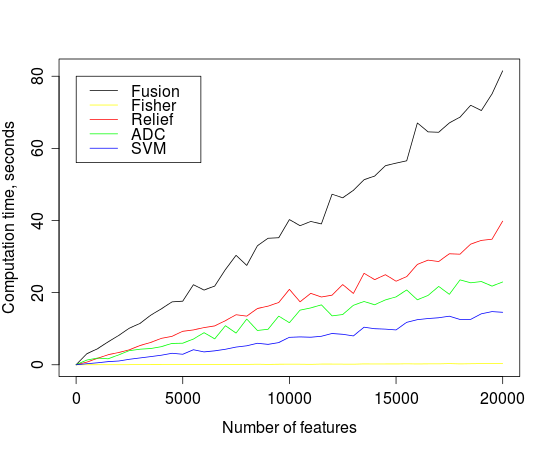
\includegraphics[width=0.7\textwidth]{images/all_performance.png}
 \caption{Pagrindinių dimensijų atrinkimo metodų skaičiavimo laikas.}
 \label{fig:visu_laikas}
\end{figure}
~\ref{fig:cgs_laikas} pavaizduotas konsensuso grupėmis grįsto dimensijų atrinkimo algoritmo skaičiavimo laiko priklausomybė nuo mėginius apibūdinančių dimensijų kiekio. Algoritmo sudėtingumas laiko atžvilgiu yra kvadratinis. Jei lyginsime su dimensijų reitingavimo algoritmais, tai šis algoritmas yra daug kartų lėtesnis.
\begin{figure}
 \centering
 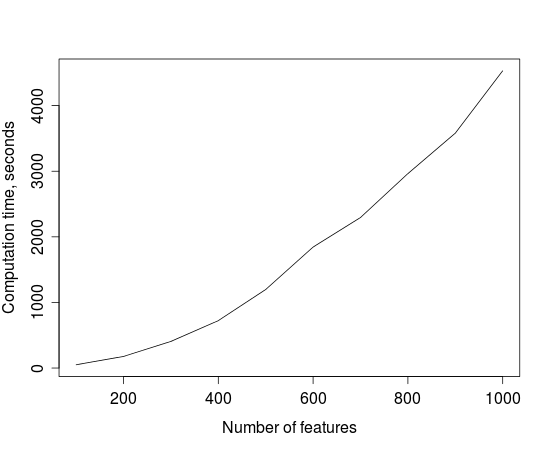
\includegraphics[width=0.7\textwidth]{images/cgs_performance.png}
 \caption{Konsensuso grupėmis grįtas dimensijų atrinkimo metodo skaičiavimo laikas.}
 \label{fig:cgs_laikas}
\end{figure}

Pagal gautus laiko priklausomybės nuo dimensijų kiekio grafikus galime daryti išvadą, kad CGS algoritmas daugiamačių duomenų dimensijų atrinkimui nėra tinkamas, nes darbo laikas yra per didelis.

\subsubsection{Klasifikavimo tikslumas}